\documentclass{article}

% Course requirement: NeurIPS preprint format. Use the course-provided neurips_2025.sty.
\usepackage[preprint]{neurips_2025}

\usepackage[utf8]{inputenc}
\usepackage[T1]{fontenc}
\usepackage[hidelinks]{hyperref}
\usepackage{float}
\usepackage{url}
\usepackage{booktabs}
\usepackage{amsfonts}
\usepackage{nicefrac}
\usepackage{microtype}
\usepackage{xcolor}
\usepackage{tabularx}
\usepackage{enumitem}
\usepackage{tikz}
\usetikzlibrary{positioning,arrows.meta,fit}

\setlist{nosep,leftmargin=1.4em}
\newcommand{\code}[1]{\texttt{#1}}

\title{Varsel Innlandet: An Agentic Digest of\\Natural Hazard Warnings for Innlandet}

% TODO: add full names before submitting.
\author{%
  Kim [Surname] \qquad Ådne [Surname] \\
  KIUA-2003, University of Inland Norway, Hamar \\
  Repository: \url{https://github.com/zetsukko/weather-demo-live}
}

\begin{document}

\maketitle

\begin{abstract}
Emergency coordinators and volunteer groups in Innlandet must follow official flood, landslide and weather warnings that are published by two agencies and revised several times a week, and today they collect them by hand. We build an agentic harness that fetches the warnings from open APIs, lets a language model write a short plain-Norwegian summary of each, and produces a daily digest whose facts are checked by code. The model writes prose only: identifiers, danger levels, areas and dates are copied from the source, and a checker rejects any digest that drops, duplicates, alters or invents a warning. We present the problem, a binary definition of success, the architecture, a walking skeleton that already runs daily, a schedule and the main risks.
\end{abstract}

\section{Problem}

\textbf{Recurring need.} Innlandet, with river systems such as Glomma, Gudbrandsdalslågen and Mjøsa, receives flood and landslide warnings from NVE and weather warnings from MET Norway repeatedly every autumn and spring. Municipal emergency coordinators (\emph{beredskapskoordinatorer}) and volunteer organisations such as the Red Cross and local search-and-rescue teams need to know which warnings apply to their area, at which level and for which period. Today this is assembled by hand from varsom.no and MET's warning pages. The work is repetitive, has no single owner, and its failures are costly: a missed update, a cancelled warning still circulated, or a wrong danger level.

\textbf{What the workflow produces.} Once a day, the harness produces \code{out/digest.json} and a readable \code{out/digest.md}. Each entry contains the official warning identifier, type, danger level, affected area and validity period, copied from the source, plus a summary of at most 60 words in plain Norwegian written by the agent. The digest carries the attribution required by the data licences and links to varsom.no. A person reads the digest and decides whether and how to pass it on; the system never sends messages.

\textbf{Users and constraints.} Users are described by role only, and the workflow processes public warnings without personal data. NVE data is licensed under NLOD~2.0; we keep the official fields intact, as NVE asks, label our text as a summary, and link to varsom.no.

\section{Definition of success}

A run is successful if and only if \code{python eval/check\_digest.py} exits with code~0. The checker compares the digest with the raw source response saved in \code{fixtures/} for that run and enforces the following binary properties:

\begin{enumerate}
  \item \textbf{Completeness:} every active warning for Innlandet in the source (danger level~$\geq 2$, valid in the period) appears in the digest exactly once, identified by its source ID.
  \item \textbf{No invention:} every \code{warning\_id} in the digest exists in the source.
  \item \textbf{Fidelity:} for each warning, \code{danger\_level}, \code{valid\_from} and \code{valid\_to} are equal to the source values.
  \item \textbf{Locality:} every warning in the digest lists Innlandet (county number~34) among its counties.
  \item \textbf{Grounded summaries:} every date, time and number that appears in a \code{summary\_no} also appears in the source record for that warning, and each summary is at most 60 words.
  \item \textbf{Attribution and privacy:} the digest contains the NVE and MET attribution strings and no e-mail addresses or phone numbers (regular-expression check).
  \item \textbf{Empty case:} if the source contains no active warning, the digest states this explicitly and contains no warnings.
\end{enumerate}

Properties 1--7 are mechanically decidable. Whether a summary is \emph{useful} and \emph{readable} is not; for the final evaluation we will add a documented LLM-as-judge rubric for these qualities, reported separately from the binary checks.

\section{Architecture}

The harness is a pipeline of five stages (Figure~\ref{fig:arch}). Only Stage~3 uses a language model; every other stage is deterministic Python using the standard library.

\begin{figure}[h]
\centering
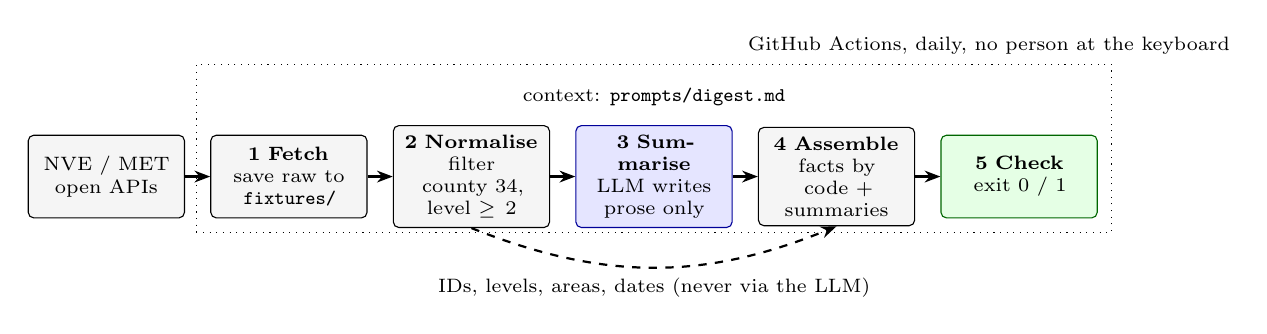
\begin{tikzpicture}[
  node distance=0.32cm,
  box/.style={draw, rounded corners=2pt, align=center, font=\scriptsize, minimum height=1.05cm, text width=1.75cm, fill=gray!8},
  llm/.style={box, fill=blue!10, draw=blue!60!black},
  chk/.style={box, fill=green!10, draw=green!40!black},
  arr/.style={-{Stealth[length=2mm]}, thick}]
  \node[box] (src) {NVE / MET\\open APIs};
  \node[box, right=of src] (s1) {\textbf{1 Fetch}\\save raw to\\\code{fixtures/}};
  \node[box, right=of s1] (s2) {\textbf{2 Normalise}\\filter county 34,\\level $\geq 2$};
  \node[llm, right=of s2] (s3) {\textbf{3 Summarise}\\LLM writes\\prose only};
  \node[box, right=of s3] (s4) {\textbf{4 Assemble}\\facts by code +\\summaries};
  \node[chk, right=of s4] (s5) {\textbf{5 Check}\\exit 0 / 1};
  \draw[arr] (src) -- (s1); \draw[arr] (s1) -- (s2); \draw[arr] (s2) -- (s3);
  \draw[arr] (s3) -- (s4); \draw[arr] (s4) -- (s5);
  \draw[arr, dashed] (s2.south) to[bend right=22] node[below, font=\scriptsize]{IDs, levels, areas, dates (never via the LLM)} (s4.south);
  \node[font=\scriptsize, above=0.12cm of s3] (ctx) {context: \code{prompts/digest.md}};
  \node[draw, dotted, fit=(s1)(s5)(ctx), inner sep=5pt, label={[font=\scriptsize]above right:GitHub Actions, daily, no person at the keyboard}] {};
\end{tikzpicture}
\caption{Pipeline of the harness. The dashed path carries all facts around the language model.}
\label{fig:arch}
\end{figure}

\textbf{Stage 1: Fetch (tool use).} \code{harness/fetch.py} calls the NVE flood-warning API (\url{https://api01.nve.no/hydrology/forecast/flood/v1.0.10}), endpoint \url{/api/Warning/County/34/1} (no dates: today, tomorrow and the day after; \code{1} = Norwegian), with an identifying \code{User-Agent}. Landslide warnings and MET MetAlerts follow after the skeleton. The raw response is saved, and \code{-{}-offline} replays a saved fixture without network access.

\textbf{Stage 2: Normalise.} The raw records are mapped to one schema (\code{source}, \code{warning\_id}, \code{type}, \code{danger\_level}, \code{area}, \code{valid\_from}, \code{valid\_to}, official text fields) and filtered to warnings that list county~34 and have level~$\geq 2$. This list is the single source of truth for all facts in the digest.

\textbf{Stage 3: Summarise (agent step).} One call to a local model, \code{llama3.2:3b} served by Ollama, receives the normalised list and a context file, \code{prompts/digest.md}, which defines the audience, the plain-language rules, the meaning of the NVE activity levels and the required JSON output (\code{warning\_id} $\rightarrow$ \code{summary\_no}). The model sees only the normalised Innlandet warnings, passed as a delimited data block that the prompt declares to be data, not instructions.

Without a configured model, or with \code{-{}-no-llm}, the stage falls back to template summaries built from the official fields, and \code{-{}-offline} replays a saved model answer, so the pipeline is reproducible without network. The local model costs nothing per run and keeps the data on our machine; the daily GitHub Actions run has no local model and uses the template fallback.

\textbf{Stage 4: Assemble.} \code{harness/assemble.py} joins the model's summaries to the Stage~2 records by \code{warning\_id} and writes \code{out/digest.json} and \code{out/digest.md} with attribution. The model's output is never trusted for facts; a summary for an unknown ID is discarded and a missing summary fails the check.

\textbf{Stage 5: Check.} \code{eval/check\_digest.py} implements Section~2; it was committed before the code it tests and the coding agent is denied edits to \code{eval/}.

\textbf{Automation.} \code{python harness/run.py} runs Stages 1--5 with one command. A GitHub Actions workflow runs it on a daily cron schedule, stores the digest as a build artifact, and fails visibly when the check fails. The local model needs no key; an optional API key would live only in a GitHub secret or a git-ignored \code{.env}. A kill switch stops the run without a digest if the API fails, the model returns invalid JSON, or more than 60 active warnings appear; \code{run.py} deletes stale output first so an old digest cannot fake a pass. Publication remains a human decision: the digest is never sent anywhere automatically.

\textbf{Development process.} Each unit of work is a task file in \code{tasks/} with an acceptance check, implemented by a coding agent on a branch and merged through a reviewed pull request; \code{CLAUDE.md} holds the rules for the agent, and corrections are logged in \code{docs/prompt-log.md}.

\section{Walking skeleton: status and first observations}

The skeleton runs end to end for NVE flood warnings and meets the four technical minimums: (1)~\code{check\_digest.py} decides properties 1--7 with exit 0/1; (2)~five stages, of which only one uses a model; (3)~tools: HTTP calls to NVE and the local model server, files and a subprocess; (4)~a GitHub Actions workflow on a daily cron schedule, whose first run on \code{master} succeeded in 11~s and stored the digest as an artifact.

\textbf{First live run (26.10).} The county endpoint returned 138 records for three days. Five of them were at level~2 (yellow) for Innlandet; they carried the same warning ID and together covered Søndre Land, Østre Toten, Vestre Toten, Gran and Sør-Aurdal, so the digest contained one warning. The local model used 747 input and 129 output tokens, and the check passed. The offline run, which replays the saved NVE response and the saved model answer, also passed.

\textbf{Failures found while building.} Building against real data exposed three problems that the plan had not anticipated. They are logged in \code{docs/prompt-log.md}:
\begin{enumerate}
  \item \emph{Wrong endpoint.} Code generated from the documentation called \code{.../v1.0.10/Warning/...} (HTTP~404); the working path is \code{.../v1.0.10/api/Warning/...}. The coding agent found this by testing the endpoint first.
  \item \emph{One record per municipality.} NVE sends one record per municipality under a shared ID; unmerged, one warning would have appeared five times and failed completeness. Stage~2 now merges by ID and stops if merged records disagree.
  \item \emph{Correct facts, poor language.} The first model summary passed every check but contained garbled Norwegian (``Flomfare er utsatt''). Checks protect facts, not language, which motivates the readability rubric and a model comparison.
\end{enumerate}
The summary also said ``søndag morgen'' on a Monday; the phrase is NVE's own, so property~5 accepted it. Grounded is not the same as up to date, which we will test with stale inputs.

\textbf{Reproducibility.} All code, context files, tasks and checks are in \url{https://github.com/zetsukko/weather-demo-live}; the README explains a normal run (\code{python harness/run.py}) and an offline run (\code{-{}-offline}).

\textbf{Does the check detect errors?} During development we changed a danger level, removed a warning, and added an invented number to a summary in a generated digest. Each change made the check fail with the corresponding property, and an ID invented by the model was discarded in Stage~4.

\section{Evaluation and safe-operation plan}

\textbf{Evaluation and stress testing.} The test set will consist of saved NVE responses with known content: typical days, the empty case, a level-3 or level-4 warning, multi-county warnings, and a case that must be rejected (a warning for another county injected into the input). The harness reports pass rates per property; readability is scored separately with a documented LLM-as-judge rubric. We will perturb the system with \emph{input perturbation} (prompt injection in \code{MainText}, malformed fields) and \emph{dependency failure} (NVE 404 or timeout, model server down), and add \emph{model variance} (two local models) if time allows.

\textbf{Safe operation.} The runtime only reads from NVE and the local model server and writes to \code{out/} and \code{fixtures/}; the coding agent may not edit \code{eval/} or read \code{.env}. Each run makes one model call with a 2000-token limit. The kill switch stops the run without a digest on an API error, invalid model output, disagreeing records, or more than 60 warnings. Nothing is sent automatically; a person decides what to pass on.

\section{Schedule}


\begin{table}[H]
\centering
\small
\begin{tabularx}{\textwidth}{@{}lX@{}}
\toprule
\textbf{When} & \textbf{Milestone} \\
\midrule
30.10 (C2) & Walking skeleton (NVE flood $\rightarrow$ local model summary $\rightarrow$ checked digest, daily run). Report submitted. \\
Week 45 & NVE landslide warnings and MET MetAlerts; test set v1 from saved fixtures. \\
Week 46 & Safe-operation measures; first stress tests; demo rehearsal. \\
Weeks 46--47 & Live demonstration. \\
Week 48 & Repairs with regression evidence; demo feedback; readability rubric. \\
3.12 & White paper submitted; commit tagged \code{exam}. \\
\bottomrule
\end{tabularx}
\end{table}

\section{Risk assessment}

\begin{table}[H]
\centering
\small
\begin{tabularx}{\textwidth}{@{}>{\raggedright\arraybackslash}p{4.2cm}X@{}}
\toprule
\textbf{Risk} & \textbf{Mitigation} \\
\midrule
No active warnings during testing & Saved fixtures incl.\ archived periods; the empty case is a required property. \\
LLM alters or invents facts & Facts bypass the model; property~5 rejects ungrounded numbers; failed check = no digest. \\
Prompt injection in warning text & Delimited data, fixed JSON schema; tested as input perturbation. \\
API change or outage & Pinned API version, fixtures and \code{-{}-offline}, explicit stop on errors. \\
Weak Norwegian from a small model & Measured with the readability rubric and a model comparison. \\
Cost or key leakage & Local model costs nothing; keys only in \code{.env} or GitHub secrets. \\
Time (two people, five weeks) & Thin skeleton first; MetAlerts dropped first if time runs short. \\
\bottomrule
\end{tabularx}
\end{table}

\newpage
\appendix

\section{Prompt log (excerpts)}

The full log is in \code{docs/prompt-log.md}. The following entries show agent output that we corrected or rejected.

\begin{itemize}[leftmargin=1.2em]
  \item \textbf{2026-10-01, task 001 plan: missing contact in the User-Agent.} The agent's plan for the MET Norway probe used a default \code{User-Agent} without contact information, which MET's terms of service require. We rejected the plan and had the agent use the repository URL instead: \code{weather-demo-live/0.1 github.com/zetsukko/weather-demo-live}. The code passed the check either way; only reading the plan caught the problem.
  \item \textbf{2026-10-01, unrequested push.} While scaffolding the repository, the agent pushed to GitHub without being asked. We now review \code{/diff} before every commit and push ourselves.
  \item \textbf{2026-10-01, credential in the git remote.} The agent noticed a GitHub token embedded in the \code{origin} remote URL and printed it in the session. We revoked the token and switched to credential-manager login. This confirmed the need to keep secrets out of anything the agent can read or print.
  \item \textbf{2026-10-26, specification contradicted the assignment.} The agent-drafted \code{SPEC.md} listed scheduling as out of scope, although the technical minimum requires an automatic part. We moved the daily run into scope and kept only hosting and notifications out.
  \item \textbf{2026-10-26, wrong licence.} The same draft gave MET Norway's licence as CC~BY~4.0 only; MET's licence page states NLOD~2.0 and CC~BY~4.0. Corrected after checking the source.
  \item \textbf{2026-10-26, facts kept away from the model.} Rather than accept a design where the model writes the whole digest, we required that identifiers, levels, areas and dates are copied by code and that the check rejects any number in a summary that is not in the source.
\end{itemize}

\section{Meeting reports}

\textbf{Meeting 2026-10-15.} \emph{Attendees:} Ådne, Kim. \emph{Done:} repository scaffolded and tagged \code{w40-scaffold}; task~001 (MET Norway probe for Hamar) merged via pull request~\#1 with the check passing; prompt log started; three problem candidates drafted. \emph{Decisions:} shortlist of a hazard warnings digest (NVE), council agenda summaries (Hamar kommune) and a campus bus brief (Entur). \emph{Next:} verify source links, book a discussion hour, choose a problem.

\textbf{Meeting 2026-10-26.} \emph{Attendees:} Ådne, Kim. \emph{Done:} remaining source links and licences verified; \code{SPEC.md} drafted for candidate~1; problem approved by the lecturer. \emph{Decisions:} hazard warnings digest chosen. The council agenda candidate was dropped because the documents may contain personal data and no reuse licence was found; the bus brief was dropped because real-time data is hard to check against a fixed source. The skeleton starts with NVE flood warnings only; Claude Haiku for the summary step; GitHub Actions for the daily run. \emph{Next:} tasks 002--004 (NVE probe, summary step, \code{run.py} and schedule) before 30.10.

\emph{Update 26.10:} no API credits were available, so the summary step was switched to a local Ollama model (\code{llama3.2:3b}).

\end{document}
